\documentclass[aspectratio=169]{beamer}

\usetheme{GRVC}

% Blocks
\setbeamerfont{block title}{size=\normalsize, series=\bfseries}
\setbeamerfont{block body}{size=\small}

% Itemize / enumerate
\setbeamerfont{itemize/enumerate body}{size=\small}
\setbeamerfont{itemize/enumerate subbody}{size=\footnotesize}


\usepackage{tikz}
\usetikzlibrary{calc}

\usepackage{amsmath,amssymb}
\usepackage{mathtools}

% Allow figures to be placed either alongside this .tex file or inside an assets/ folder
\graphicspath{{./}{assets/}{assets/figures/}{figures/}}

% Partner logo helper (used for consortium slides)
\newcommand{\GRVCpartnerlogo}[1]{%
  \includegraphics[width=0.16\textwidth,height=1.5cm,keepaspectratio]{#1}%
}

% Set a transparent background image for all frames
\setbeamertemplate{background}{%
  \begin{tikzpicture}[remember picture,overlay]
    \node[opacity=0.95, at=(current page.center)] {%
      \includegraphics[width=\paperwidth,height=\paperheight]{assets/background.png}%
    };
  \end{tikzpicture}%
}

\title{GRVC Lab\\Biweekly seminars}
\author{Abdalraheem Abdullah Yousef Ijieh}
% \institute{GRVC Robotics Labs}
\date{16 Enero 2026}

\begin{document}

% Title slide (first slide) includes GRVC logo at lower-left by design
\begin{frame}[plain]
  \titlepage
\end{frame}


% Example: section divider with project logo (top-right)
\GRVCsectionframe[assets/tema\_logo.png]{Trusted extremely precise mapping and prediction for emergency management}

% --- Consortium partners (logos are sourced from the official TEMA partners page) ---
{\setbeamertemplate{background}{%
  \begin{tikzpicture}[remember picture,overlay]
    \fill[GRVCCYAN] (current page.south west) rectangle (current page.north east);
  \end{tikzpicture}}
  }


{
\GRVCsetprojectlogo{assets/tema_logo.pdf}
\begin{frame}{TEMA in a Nutshell}
  \begin{columns}[T,onlytextwidth]
    % ---------------- Left column: Partners ----------------
    \column{0.4\textwidth}
      \centering
      {\bfseries Consortium partners}\par\vspace{0.4em}

      % tighten spacing so it fits nicely
      \setlength{\tabcolsep}{3pt}
      \renewcommand{\arraystretch}{0.95}

      \begin{tabular}{ccccc}
        \GRVCpartnerlogo{assets/partners/auth.png} &
        \GRVCpartnerlogo{assets/partners/atos.png} &
        \GRVCpartnerlogo{assets/partners/brk.png} &
        \GRVCpartnerlogo{assets/partners/dmalian.png} &
        \GRVCpartnerlogo{assets/partners/engineering.png} \\
        \GRVCpartnerlogo{assets/partners/fraunhofer_hhi.png} &
        \GRVCpartnerlogo{assets/partners/dlr.png} &
        \GRVCpartnerlogo{assets/partners/itu.png} &
        \GRVCpartnerlogo{assets/partners/kamk.png} &
        \GRVCpartnerlogo{assets/partners/kaj.png} \\
        \GRVCpartnerlogo{assets/partners/kemea.png} &
        \GRVCpartnerlogo{assets/partners/latitudo40.png} &
        \GRVCpartnerlogo{assets/partners/nelen_schuurmans.png} &
        \GRVCpartnerlogo{assets/partners/northdocks.png} &
        \GRVCpartnerlogo{assets/partners/plus.png} \\
        \GRVCpartnerlogo{assets/partners/ras.png} &
        \GRVCpartnerlogo{assets/partners/tecnosylva.png} &
        \GRVCpartnerlogo{assets/partners/lisbon_council.png} &
        \GRVCpartnerlogo{assets/partners/use.png} &
        \GRVCpartnerlogo{assets/partners/unime.png} \\
      \end{tabular}

    % ---------------- Right column: At a glance ----------------
    \column{0.54\textwidth}
    \centering 
    {\bfseries \large TEMA at a glance}\par\vspace{0.3em}
    \centering
    \begin{tabular}{ccc}
      {20 Partners} & {4 Years} & {11 M\texteuro}
    \end{tabular}
    \par\vspace{0.7em}
    \raggedright

    % Optional: also shrink block title/body a touch (local to this frame/column)
    \setbeamerfont{block title}{size=\footnotesize,series=\bfseries}
    \setbeamerfont{block body}{size=\scriptsize}
    \setbeamerfont{itemize/enumerate body}{size=\scriptsize}

    \begin{block}{Mission}
      Deliver actionable situational awareness for disaster response by turning multi-source data into decision-ready information.
    \end{block}

    \vspace{-0.3em}
    \begin{itemize}
      \setlength{\itemsep}{0.35em}
      \item Bring real-time situational data to responders and relevant end-users.
      \item Support operational decision-making during evolving incidents.
      \item Transferable across hazards (e.g., flood, wildfire) and geographic regions.
    \end{itemize}

  \end{columns}
\end{frame}
\GRVCclearprojectlogo
}

%%%%%%%%%%%%%%%%%%%%%%%%%%%%%%%%%%%%%%%%%%%%%%%
% --- TEMA technologies (USE highlighted) ---
{
\GRVCsetprojectlogo{assets/tema_logo.pdf}

% Robust highlighting (avoid table-row coloring issues on beamer themes)
\newcommand{\USEtech}[1]{\textbf{\textcolor{GRVCCyan}{#1}}}

\begin{frame}{TEMA technologies}
  \scriptsize
  \setlength{\tabcolsep}{2pt}
  \renewcommand{\arraystretch}{0.95}
  \tiny
  \begin{columns}[T,onlytextwidth]
    % ---------------- TFA ----------------
    \column{0.4\textwidth}
    {\bfseries Trustworthy Federated Analytics}\par\vspace{0.25em}
    \begin{tabular}{@{}p{0.24\linewidth}p{0.74\linewidth}@{}}
      \textbf{ID} & \textbf{Technology}\\ \hline
      TFA-tech-01 & Concept discovery for latent space interpretability of deep neural networks\\
      TFA-tech-02 & Human-comprehensible presentation of concept-based explanations\\
      TFA-tech-03 & DNN robustness\\
      TFA-tech-04 & Explainability for transformer base neural networks\\
      TFA-tech-05 & Fire/smoke/flood/person detection\\
      TFA-tech-06 & Fire/flood/background segmentation\\
      TFA-tech-07 & Person re-identification\\
      TFA-tech-08 & Satellite-based flood detection and assessment\\
      TFA-tech-09 & Satellite-based Forest fire detection and assessment\\
      TFA-tech-10 & Privacy preservation during visual analysis\\
      TFA-tech-11 & Geo-social media analysis\\
      TFA-tech-12 & Sentiment analysis for short texts\\
      TFA-tech-13 & Contrastive image-language models\\
      TFA-tech-14 & Federated Learning\\
      TFA-tech-15 & Data scarcity, synthetic data generation pipeline\\
    \end{tabular}

    % ---------------- PDM ----------------
    \column{0.29\textwidth}
    {\bfseries Phenomenon Prediction and Decision-Macking}\par\vspace{0.25em}
    \begin{tabular}{@{}p{0.44\linewidth}p{0.54\linewidth}@{}}
      \textbf{ID} & \textbf{Technology}\\ \hline
      PDM-tech-01 & Forest Fire Simulation\\
      PDM-tech-02 & 3Di Hydrodynamic simulation\\
      PDM-tech-03 & Realistic 3D smoke modelling and fire detection\\
      \USEtech{PDM-tech-04} & \USEtech{Drone planning}\\
      \USEtech{PDM-tech-05} & \USEtech{Information fusion}\\
      PDM-tech-06 & Data-fusion-based decision support and process triggering\\
    \end{tabular}

    % ---------------- SV ----------------
    \column{0.24\textwidth}
    {\bfseries Simulation and Visualization}\par\vspace{0.25em}
    \begin{tabular}{@{}p{0.44\linewidth}p{0.54\linewidth}@{}}
      \textbf{ID} & \textbf{Technology}\\ \hline
      \USEtech{SV-tech-01} & \USEtech{Drone-based image and data acquisition}\\
      SV-tech-02 & Digital Enabler\\
      SV-tech-03 & 3D computer vision (SfM)/ Photogrammetry\\
      SV-tech-04 & Geovisual Analytics\\
      SV-tech-05 & Geospatial information retrieval\\
      SV-tech-06 & Extended Reality-based interactive visualisation system\\
      SV-tech-07 & Smartdesk\\
    \end{tabular}
  \end{columns}

  \vspace{0.4em}
  \tiny \textcolor{GRVCCyan}{\rule{0.9em}{0.9em}} \; \textit{University of Seville (USE) technologies: SV-tech-01, PDM-tech-04, PDM-tech-05.}
\end{frame}
\GRVCclearprojectlogo
}





% ------------------------------------------------------------
% Information Fusion (PDM-tech-05) — University of Seville (USE)
% ------------------------------------------------------------
\GRVCsectionframe[assets/tema\_logo.png]{Information fusion (PDM-tech-05)}

{
\GRVCsetprojectlogo{assets/tema_logo.pdf}

% Clean background for technical content (better readability than a photo background)
\setbeamertemplate{background}{%
  \begin{tikzpicture}[remember picture,overlay]
    \fill[GRVCBlue] (current page.south west) rectangle (current page.north east);
  \end{tikzpicture}%
}


\begin{frame}{Information fusion: storyline}
  \small
  \begin{itemize}\itemsep0.4em
    \item Natural Disaster Management (NDM) produces \textbf{many signals} (UAV, satellite, models, geo-social), often \textbf{asynchronous} and \textbf{contradictory}.
    \item PDM-tech-05 turns these signals into a \textbf{single, continuously updated operational picture}.
    \item Two primary outputs:
      \begin{itemize}\itemsep0.2em
        \item \textbf{Occupancy Grid Map (OGM)}: disaster status (Flood \& Fire) as a probabilistic map.
        \item \textbf{Object Presence Map (OPM)}: multi-object tracking (people/vehicles) with uncertainty.
      \end{itemize}
    \item Later: we demonstrate the platform with a \textbf{flood case study} (Ahrtal), aligned with the draft paper.
  \end{itemize}
\end{frame}

\begin{frame}{Motivation: why we need information fusion}
  \begin{columns}[T,onlytextwidth]
    \column{0.58\textwidth}
      \small
      \begin{itemize}\itemsep0.5em
        \item In disasters, the bottleneck is not data availability, but \textbf{coherence}.
        \item UAV: detailed but local and intermittent.
        \item Satellite: wide-area but delayed and sometimes uncertain.
        \item Simulations: predictive but model-dependent.
        \item Geo-social: fast but noisy and biased.
      \end{itemize}
      \vspace{0.4em}
      \begin{block}{Goal}
        Provide \textbf{one operational picture} that updates whenever new evidence arrives.
      \end{block}
    \column{0.40\textwidth}
      \centering
      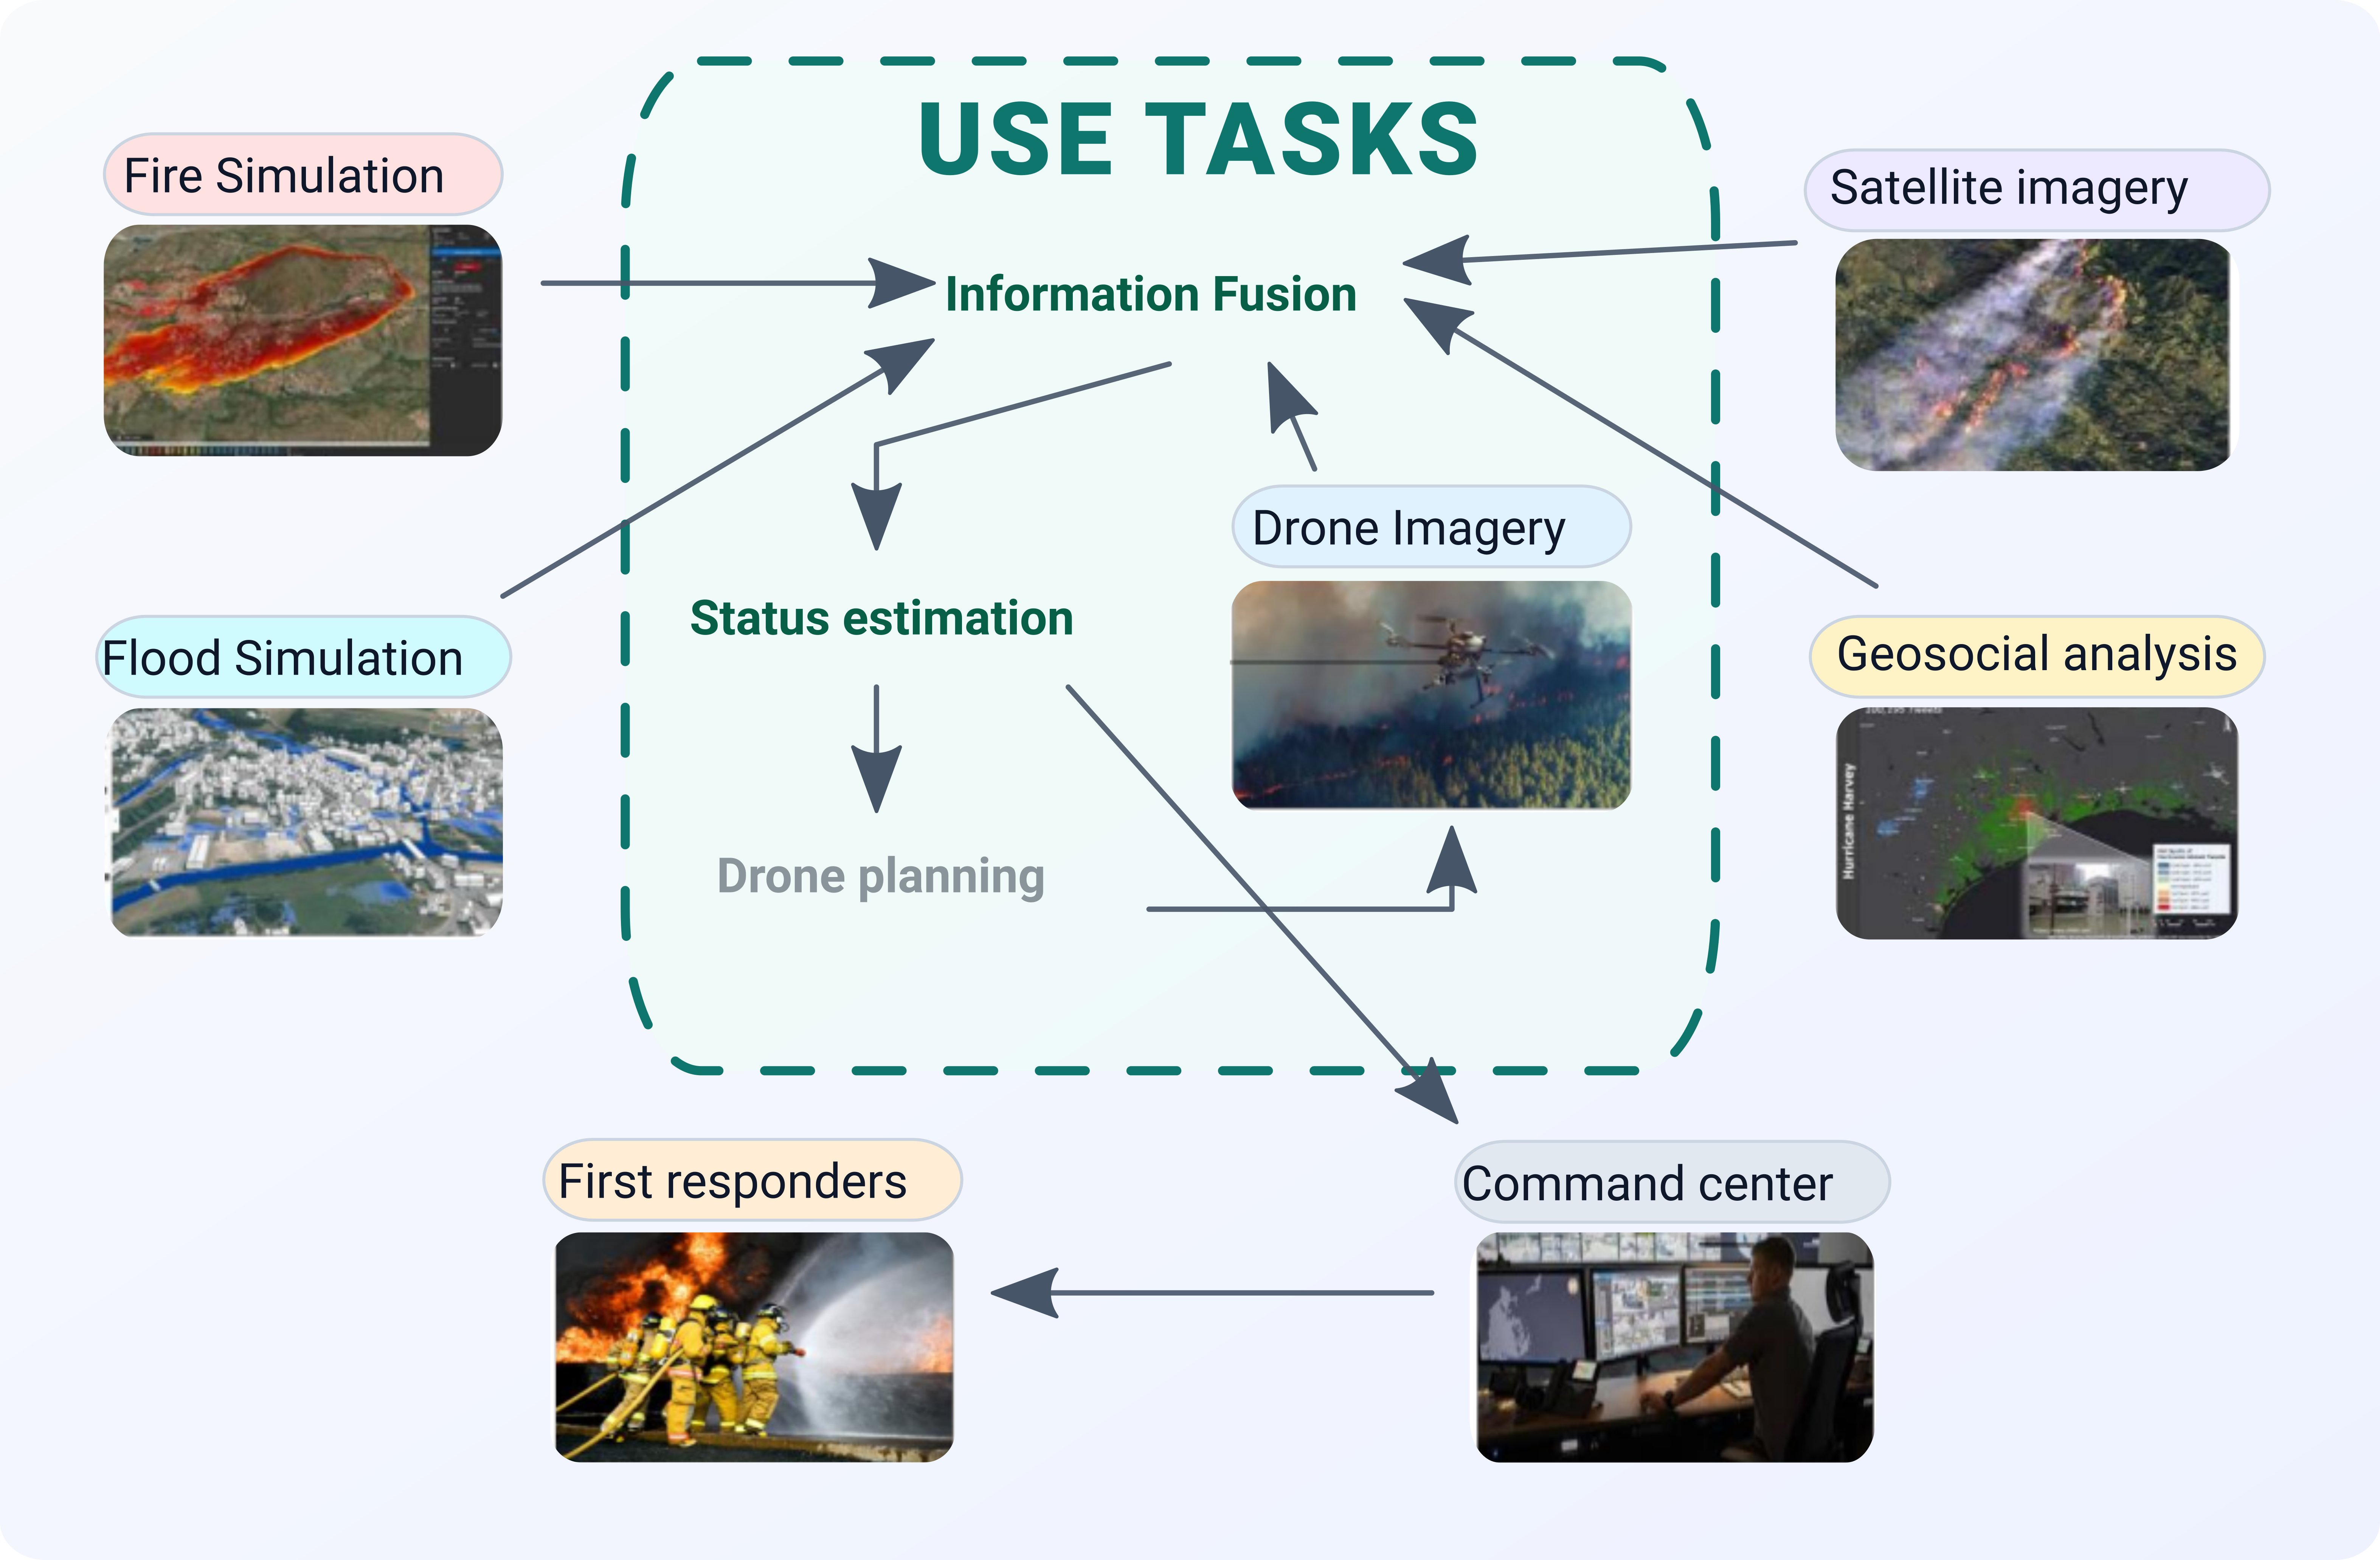
\includegraphics[width=\linewidth,height=0.72\textheight,keepaspectratio]{enhanced_end_to_end_scheme.png}
  \end{columns}
\end{frame}

\begin{frame}{Key challenges addressed by PDM-tech-05}
  \small
  \begin{itemize}\itemsep0.6em
    \item \textbf{Asynchrony:} different refresh rates and latencies (seconds to hours).
    \item \textbf{Heterogeneity:} masks, grids, point detections, text-derived signals, forecasts.
    \item \textbf{Uncertainty:} every source is imperfect; disagreement is normal.
    \item \textbf{Georeferencing:} mobile sensors + terrain $\Rightarrow$ spatial alignment is non-trivial.
    \item \textbf{Dynamics:} evolving hazard fronts and moving objects $\Rightarrow$ temporal consistency matters.
  \end{itemize}
\end{frame}

\begin{frame}{What the Information Fusion platform does}
  \begin{columns}[T,onlytextwidth]
    \column{0.55\textwidth}
      \small
      \begin{enumerate}\itemsep0.45em
        \item \textbf{Ingest} NGSI-LD entities (measurements + predictions).
        \item \textbf{Georeference} observations into a common map frame (AOI grid).
        \item \textbf{Fuse} evidence probabilistically (event-driven updates).
        \item \textbf{Track} objects over time (OPM).
        \item \textbf{Publish} updated products to SmartDesk and downstream services.
      \end{enumerate}
      \vspace{0.3em}
      \begin{block}{Platform property}
        Same engine across hazards; hazard-specificity enters via input models and the OGM semantics (Flood/Fire).
      \end{block}
    \column{0.43\textwidth}
      \centering
      \includegraphics[width=\linewidth,height=0.75\textheight,keepaspectratio]{INTERACTION_DIAGRAM.png}
  \end{columns}
\end{frame}

\begin{frame}{Two primary outputs: OGM and OPM}
  \small
  \begin{columns}[T,onlytextwidth]
    \column{0.50\textwidth}
      \begin{block}{Output 1: Occupancy Grid Map (OGM)}
        \begin{itemize}\itemsep0.35em
          \item Discretize the AOI into grid cells.
          \item Each cell stores a probability of occupancy:
          \begin{itemize}\itemsep0.2em
            \item \textbf{Flood OGM:} probability of water presence.
            \item \textbf{Fire OGM:} probability of fire/smoke/burnt area presence.
          \end{itemize}
          \item Updated from measurements \& predictions using Bayesian log-odds.
        \end{itemize}
      \end{block}

    \column{0.50\textwidth}
      \begin{block}{Output 2: Object Presence Map (OPM)}
        \begin{itemize}\itemsep0.35em
          \item Tracks persons/vehicles in geodetic coordinates.
          \item Data association (Hungarian) + state estimation (Kalman).
          \item Produces stable trajectories and uncertainty, not flickering detections.
        \end{itemize}
      \end{block}

      \vspace{0.4em}
      \begin{block}{Operational view (web app)}
        OGM + OPM are served as the evolving operational picture to the command center.
      \end{block}
  \end{columns}
\end{frame}

\begin{frame}{Web app and services architecture (deployment view)}
  \centering
  \includegraphics[width=\textwidth,height=0.86\textheight,keepaspectratio]{web_app_diagram.png}
\end{frame}

\begin{frame}{Core engine: asynchronous occupancy-grid mapping}
  \begin{columns}[T,onlytextwidth]
    \column{0.46\textwidth}
      \small
      \begin{itemize}\itemsep0.5em
        \item The OGM is updated \textbf{whenever} new evidence arrives.
        \item Measurements: update occupancy via inverse sensor models.
        \item Predictions: propagate or bias occupancy using forecast evidence.
        \item Asynchrony is handled naturally (no need to wait for all sources).
      \end{itemize}
    \column{0.52\textwidth}
      \centering
      \includegraphics[width=\linewidth,height=0.78\textheight,keepaspectratio]{asyncapproach.png}
  \end{columns}
\end{frame}

% -----------------------------
% OGM: Fundamentals + equations
% -----------------------------
\begin{frame}{OGM formalism: probability and log-odds}
  \scriptsize
  \setlength{\abovedisplayskip}{2pt}
  \setlength{\belowdisplayskip}{2pt}

  Discretize the AOI into cells $m_i$ and maintain an occupancy probability $p_t(i)=P(m_i \text{ occupied at time } t)$.

  \vspace{0.3em}
  \begin{align*}
    \ell_t(i) &= \log \frac{p_t(i)}{1-p_t(i)} \qquad\text{(log-odds)}\\
    p_t(i) &= \sigma(\ell_t(i))=\frac{1}{1+e^{-\ell_t(i)}} \qquad\text{(logistic)}\\
    \ell_0(i) &= \log \frac{P(m_i)}{1-P(m_i)} \qquad\text{(prior, typically }P(m_i)=0.5\text{ inside AOI)}
  \end{align*}

  \begin{block}{Why log-odds?}
    Numerical stability and additive updates across asynchronous sources.
  \end{block}
\end{frame}

\begin{frame}{OGM fusion rule: Bayesian log-odds update}
  \scriptsize
  \setlength{\abovedisplayskip}{2pt}
  \setlength{\belowdisplayskip}{2pt}

  For an incoming observation $z_t$ (from any source) and platform state $x_t$:

  \begin{align*}
    \ell_t(i) &= \ell_{t^-}(i) + \log \frac{P(m_i \mid z_t, x_t)}{1-P(m_i \mid z_t, x_t)} - \ell_0(i)\\
              &= \ell_{t^-}(i) + \underbrace{\log\frac{P(z_t\mid m_i,x_t)}{P(z_t\mid \neg m_i,x_t)}}_{\text{evidence from source}} - \ell_0(i)
  \end{align*}

  \begin{block}{Interpretation}
    Each source provides a per-cell occupancy probability (or likelihood), which is converted into a log-odds increment and added to the current map.
  \end{block}
\end{frame}

\begin{frame}{Fusion of measurements vs. predictions}
  \small
  \begin{itemize}\itemsep0.6em
    \item \textbf{Measurements} (UAV/satellite/geo-social) update the current OGM via inverse sensor models.
    \item \textbf{Predictions} (e.g., hydrodynamics, fire simulation) encode forecast evidence and can be fused:
      \begin{itemize}\itemsep0.3em
        \item as additional log-odds evidence, or
        \item via \textbf{logit pooling} (weighted combination in log-odds space).
      \end{itemize}
    \item The platform remains generic: source-specificity enters only through the mapping from raw outputs to $p^{(s)}_t(i)$.
  \end{itemize}
\end{frame}

% -----------------------------
% Flood: measurement models
% -----------------------------
\begin{frame}{Flood measurement model: UAV flood segmentation}
  \tiny
  \setlength{\abovedisplayskip}{1pt}
  \setlength{\belowdisplayskip}{1pt}

  Let the segmentation provide per-pixel flood scores $s_k^{uav}\in[0,1]$ for pixels $k$ projected into grid cell $i$.

  \begin{align*}
    \bar{s}^{uav}_i &= \frac{1}{n_i}\sum_{k \in K_i} s^{uav}_k \\
    p^{uav}_i &= p^{uav}_{\min} + \left(p^{uav}_{\max}-p^{uav}_{\min}\right)\bar{s}^{uav}_i \\
    \delta\ell^{uav}(i) &= \log\frac{p^{uav}_i}{1-p^{uav}_i}, \qquad \ell_t(i)=\ell_{t^-}(i)+\delta\ell^{uav}(i)
  \end{align*}

  \begin{block}{Notes}
    $\;p^{uav}_{\min},p^{uav}_{\max}$ encode trust in the segmentation (avoid overconfidence).
  \end{block}
\end{frame}

\begin{frame}{Flood measurement model: satellite flood extent}
  \tiny
  \setlength{\abovedisplayskip}{1pt}
  \setlength{\belowdisplayskip}{1pt}

  Satellite products provide a per-cell flood probability (or a mask mapped to probability) $m^{sat}_i$.

  \begin{align*}
    p^{sat}_i &= \operatorname{clip}\left(m^{sat}_i,\varepsilon,1-\varepsilon\right)\\
    \delta\ell^{sat}(i) &= \log\frac{p^{sat}_i}{1-p^{sat}_i}, \qquad \ell_t(i)=\ell_{t^-}(i)+\delta\ell^{sat}(i)
  \end{align*}

  \begin{block}{Notes}
    $\varepsilon$ prevents infinite log-odds; confidence can be source-dependent (clouds, resolution, latency).
  \end{block}
\end{frame}

\begin{frame}{Flood measurement model: geo-social hotspots}
  \tiny
  \setlength{\abovedisplayskip}{1pt}
  \setlength{\belowdisplayskip}{1pt}

  Geo-social analytics yields a spatial score from activity and relevance signals (normalized per AOI):

  \begin{align*}
    s^{soc}_t(i) &= w_c\,\tilde{c}_t(i) + w_r\,\tilde{r}_t(i), \qquad w_c+w_r=1 \\
    p^{soc}_t(i) &= \varepsilon + (1-2\varepsilon)\, s^{soc}_t(i) \\
    \delta\ell^{soc}(i) &= \log\frac{p^{soc}_t(i)}{1-p^{soc}_t(i)}, \qquad \ell_t(i)=\ell_{t^-}(i)+\delta\ell^{soc}(i)
  \end{align*}

  \begin{block}{Notes}
    Geo-social is treated as \textbf{uncertain evidence} (use conservative bounds).
  \end{block}
\end{frame}

% -----------------------------
% Flood: prediction fusion
% -----------------------------
\begin{frame}{Flood prediction fusion: hydrodynamic depth (3Di)}
  \tiny
  \setlength{\abovedisplayskip}{1pt}
  \setlength{\belowdisplayskip}{1pt}

  Convert predicted water depth $h_i$ into occupancy probability via a logistic mapping:

  \begin{align*}
    p^{hyd}_i &= \varepsilon + (1-2\varepsilon)\,\frac{1}{1+\exp\left(-\frac{h_i-h_{50}}{s}\right)} \\
    \ell^{hyd}_i &= \log\frac{p^{hyd}_i}{1-p^{hyd}_i}
  \end{align*}

  \textbf{Logit pooling (weighted fusion in log-odds space):}
  \begin{align*}
    \ell^{new}_i &= (1-\alpha_{hyd})\,\ell^{ogm}_i + \alpha_{hyd}\,\ell^{hyd}_i
  \end{align*}

  \begin{block}{Notes}
    $\alpha_{hyd}\in[0,1]$ controls reliance on prediction vs. accumulated evidence.
  \end{block}
\end{frame}

\begin{frame}{Fusing predictive outputs in a generic way}
  \scriptsize
  \setlength{\abovedisplayskip}{2pt}
  \setlength{\belowdisplayskip}{2pt}

  Prediction sources provide $p^{pred}_i$ on the same grid (e.g., fire arrival time, binary forecast, propagation probability).

  \begin{align*}
    p^{pred}_i &\rightarrow \ell^{pred}_i = \log\frac{p^{pred}_i}{1-p^{pred}_i} \\
    \ell^{new}_i &= (1-\alpha_{pred})\,\ell^{ogm}_i + \alpha_{pred}\,\ell^{pred}_i \quad \text{(logit pooling)}
  \end{align*}

  \begin{block}{Key point}
    Predictions are fused as \textbf{evidence}, not as immutable truth; the same mechanism applies to floods and wildfires.
  \end{block}
\end{frame}

\begin{frame}{Extending beyond floods: fire occupancy (Maps4Fire)}
  \small
  \begin{itemize}\itemsep0.6em
    \item Same OGM formalism; semantics change to \textbf{fire/smoke/burnt area occupancy}.
    \item Example: combine fire front and burnt-area evidence:
      \[
        p_m(i)=w_{fire}\,p_{fire}(i)+w_{burnt}\,p_{burnt}(i),\qquad w_{fire}+w_{burnt}=1
      \]
    \item Update $\ell_t(i)$ using the same log-odds / pooling rules.
  \end{itemize}
\end{frame}

% -----------------------------
% OPM: tracking equations
% -----------------------------
\begin{frame}{OPM: state, motion model, and prediction}
  \scriptsize
  \setlength{\abovedisplayskip}{2pt}
  \setlength{\belowdisplayskip}{2pt}

  Track $k$ maintains a 6D state (geodetic position + velocity):
  \[
    x_{t,k}=\begin{bmatrix}\lambda&\phi&h&\dot{\lambda}&\dot{\phi}&\dot{h}\end{bmatrix}^{\!\top}
  \]

  Constant-velocity prediction transition:
  \[
    x_{t+1,k}=A x_{t,k} + w_t,\quad
    A=\begin{bmatrix}
      1&0&0&\Delta t&0&0\\
      0&1&0&0&\Delta t&0\\
      0&0&1&0&0&\Delta t\\
      0&0&0&1&0&0\\
      0&0&0&0&1&0\\
      0&0&0&0&0&1
    \end{bmatrix}
  \]

  Prediction step:
  \[
    \hat{x}_{t|t-1,k}=A\hat{x}_{t-1|t-1,k},\qquad
    P_{t|t-1,k}=AP_{t-1|t-1,k}A^\top+Q
  \]
\end{frame}

\begin{frame}{OPM data association: gating and Hungarian assignment}
  \scriptsize
  \setlength{\abovedisplayskip}{2pt}
  \setlength{\belowdisplayskip}{2pt}

  For detection $j$ at position $p_{t,j}$ and predicted track position $\hat{p}_{t|t-1,k}$:
  \[
    d_{k,j}=d_{hav}(\hat{p}_{t|t-1,k},p_{t,j})
  \]

  Cost matrix for assignment (example):
  \[
    C_{k,j}=\alpha\,\frac{d_{k,j}}{r_{gate}}+\beta\,(1-c^{det}_{t,j})
  \]

  \begin{block}{Association}
    Apply gating ($d_{k,j}<r_{gate}$) then solve the assignment with the Hungarian algorithm.
  \end{block}
\end{frame}

\begin{frame}{OPM state correction: confidence-aware Kalman update}
  \scriptsize
  \setlength{\abovedisplayskip}{2pt}
  \setlength{\belowdisplayskip}{2pt}

  Measurement model (position):
  \[
    z_{t,j}=H x_{t,k}+v_t,\quad
    H=\begin{bmatrix}1&0&0&0&0&0\\0&1&0&0&0&0\\0&0&1&0&0&0\end{bmatrix}
  \]

  Confidence-aware measurement noise:
  \[
    R_{t,j}=\frac{1}{\max(c^{det}_{t,j},\varepsilon_c)}\,R_{base}
  \]

  Kalman update:
  \[
    S=HPH^\top+R,\quad K=PH^\top S^{-1},\quad
    \hat{x}_{t|t}=\hat{x}_{t|t-1}+K(z-H\hat{x}_{t|t-1})
  \]
\end{frame}

% -----------------------------
% Case study (later in the story)
% -----------------------------
\begin{frame}{Case study focus: floods as a demonstrator (Ahrtal)}
  \small
  \begin{itemize}\itemsep0.6em
    \item The platform is generic (Flood \& Fire); we demonstrate end-to-end behavior on a flood event.
    \item Floods stress-test multimodality: UAV segmentation, satellite extent, geo-social signals, hydrodynamic prediction.
    \item Narrative to show: \textbf{uncertain initialization} $\rightarrow$ \textbf{progressive refinement} as evidence arrives.
  \end{itemize}
\end{frame}

\begin{frame}{Key takeaways}
  \small
  \begin{itemize}\itemsep0.6em
    \item \textbf{Generic platform} for NDM: consistent handling of heterogeneous, asynchronous evidence.
    \item \textbf{Two primary outputs:} OGM (Flood/Fire status) and OPM (multi-object tracking).
    \item \textbf{Operationalization:} event-driven service + web app operator cockpit + NGSI-LD interoperability.
    \item \textbf{USE loop:} Fusion $\rightarrow$ Drone planning $\rightarrow$ Drone acquisition $\rightarrow$ Fusion.
  \end{itemize}
\end{frame}

\GRVCclearprojectlogo
} 
\end{document}
